% ---- pg-112 （书页 100） ----

偏差(列)向量为 $\mathbf{d}'_{1}=[-2,1,1], \mathbf{d}'_{2}=[1,0,-1]$ 和 $\mathbf{d}'_{3}=[0,1,-1]$. 由于 $\mathbf{d}_{3}=\mathbf{d}_{1}+2\mathbf{d}_{2}$, 有列退化(注意也有行退化). 这意味着偏差向量之一, 例如 $\mathbf{d}_{3}$, 位于其他两个剩余向量生成的平面内. 因此, 三维体积是零. 这情况如\hyperref[fig:3.9]{图 3.9} 所示, 并可以通过证明 $|\mathbf{S}|=0$ 作代数检验. 我们有

\begin{mvfigure}
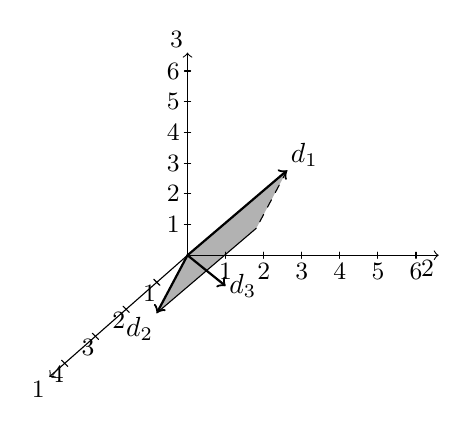
\begin{tikzpicture}[scale=0.78,line join=round,line cap=round]
% 坐标基: 轴1 单位向量 (-0.50,-0.44), 轴2 单位向量 (0.62,0), 轴3 单位向量 (0,0.50)
% 向量: d1=(-2,1,1) d2=(1,0,-1) d3=(0,1,-1)
% 阴影: 由 d1 与 d2 张成的平行四边形
\fill[black!30] (0,0) -- (1.62,1.38) -- (1.12,0.44) -- (-0.50,-0.94) -- cycle;
\draw[dashed] (1.62,1.38) -- (1.12,0.44);
\draw (1.12,0.44) -- (-0.50,-0.94);
% 轴2
\draw[->] (0,0) -- (4.09,0);
\foreach \k in {1,...,6} {
  \draw (0.62*\k,-0.05) -- (0.62*\k,0.05);
  \node[below,inner sep=1.5pt,font=\small] at (0.62*\k,-0.05) {\k};
}
\node[below left,inner sep=1.5pt,font=\small] at (4.09,0) {2};
% 轴3
\draw[->] (0,0) -- (0,3.30);
\foreach \k in {1,...,6} {
  \draw (-0.05,0.5*\k) -- (0.05,0.5*\k);
  \node[left,inner sep=1.5pt,font=\small] at (-0.05,0.5*\k) {\k};
}
\node[above left,inner sep=1.5pt,font=\small] at (0,3.30) {3};
% 轴1
\draw[->] (0,0) -- (-2.25,-1.98);
\foreach \k in {1,...,4} {
  \draw (-0.50*\k+0.05,-0.44*\k-0.05) -- (-0.50*\k-0.05,-0.44*\k+0.05);
}
\node[font=\small] at (-0.62,-0.62) {1};
\node[font=\small] at (-1.12,-1.06) {2};
\node[font=\small] at (-1.62,-1.50) {3};
\node[font=\small] at (-2.12,-1.94) {4};
\node[below left,inner sep=1.5pt,font=\small] at (-2.25,-1.98) {1};
% 向量
\draw[->,thick] (0,0) -- (1.62,1.38) node[above right,inner sep=1pt] {$d_{1}$};
\draw[->,thick] (0,0) -- (-0.50,-0.94) node[below left,inner sep=1pt] {$d_{2}$};
\draw[->,thick] (0,0) -- (0.62,-0.50) node[right,inner sep=1pt] {$d_{3}$};
\end{tikzpicture}
\phantomsection\label{fig:3.9}\mvcap{图 3.9\quad 三维体积为零的一个实例($|\mathbf{S}|=0$)}
\end{mvfigure}

\[
\underset{(3\times3)}{\mathbf{S}}=\begin{bmatrix}3&-\dfrac{3}{2}&0\\[3pt]-\dfrac{3}{2}&1&\dfrac{1}{2}\\[3pt]0&\dfrac{1}{2}&1\end{bmatrix}
\]

并从定义 2A.24,
\begin{align*}
|\mathbf{S}|&=3\begin{vmatrix}1&\frac{1}{2}\\\frac{1}{2}&1\end{vmatrix}(-1)^{2}+\left(-\frac{3}{2}\right)\begin{vmatrix}-\frac{3}{2}&\frac{1}{2}\\0&1\end{vmatrix}(-1)^{3}+0\begin{vmatrix}-\frac{3}{2}&1\\0&\frac{1}{2}\end{vmatrix}(-1)^{4}\\
&=3\times\left(1-\frac{1}{4}\right)+\frac{3}{2}\times\left(-\frac{3}{2}-0\right)+0=\frac{9}{4}-\frac{9}{4}=0\qquad\blacksquare
\end{align*}

当用电子化方式传送和接收大的数据集时, 研究者有时会意外发现零广义方差的情况, 使得 $\mathbf{S}$ 没有逆. 我们曾遇到这样的情况, 而且在未弄明情况以前会带来困难. 例如, 当数据是许多测验分数并且研究者已经把是其他变量之和的变量也包含进来时, 一个奇异的协方差矩阵就出现了. 比如说, 代数分数与几何分数可以合起来给出一个总的数学分数, 或随堂期中测验和期末考试分数加起来得到总成绩. 再如, 许多化学制品的总重量已包括了每个分量的重量.

由诸原始变量之和产生新变量, 并把它们都包含在数据集中, 这种常见做法会使我们失去了大量时间, 因而必须强调这种后果.

\noindent\textbf{例 3.10}\quad (产生的新变量会导致零广义方差)

考虑数据矩阵
\[
\mathbf{X}=\begin{bmatrix}1&9&10\\4&12&16\\2&10&12\\5&8&13\\3&11&14\end{bmatrix}
\]
其中第三列是第一、二列之和. 这些数据分别是钟点雇工和全时雇工每天成功的电话求职个数. 这样, 第三列是每天成功求职的总数.

证明广义方差 $|\mathbf{S}|=0$, 并确定数据的自然相关性.

我们求得每一项为 $x_{ik}-\bar{x}_{k}$ 的被均值修正的数据矩阵, 是
\[
\mathbf{X}-\mathbf{1}\bar{\mathbf{x}}'=\begin{bmatrix}-2&-1&-3\\1&2&3\\-1&0&-1\\2&-2&0\\0&1&1\end{bmatrix}
\]
